% !TEX root = ../main.tex
\subsection{Acceptance Correction Results}
\label{14.20::acceptance_correction_results}
    % TODO. Remove FMT3 tracks from here onward.
    DC and FMT acceptances were obtained by following the procedure described in Section \ref{13.13::acc_corr}.
    In this section, we'll study the acceptance percentage for each electron and hadronic variable.
    These numbers represent the percentage of thrown particles that were detected by the DC, 2 FMT layers, and 3 FMT layers in the \texttt{gemc} simulation.

    Since they represent the acceptance percentage, all plots display a calculated division as follows
    \begin{equation}
        y_\text{acc} = \frac{y_d}{y_t},
        \label{eq::14.20::acc}
    \end{equation}
    where $y_\text{acc}$ is the percentage of accepted particles, $y_d$ is the number of detected particles by the studied detector, and $y_t$ is the number of particles thrown by LEPTO.

    Then, to propagate the error of $y_d$ ($e_d$) and $y_t$ ($e_t$) to $y_\text{acc}$ ($e_\text{acc}$), we get
    \begin{align}
        e_\text{acc} &= \delta \left(\frac{y_r}{y_t}\right)
        \nonumber \\
        &= y_\text{acc} \cdot \sqrt{
            \left( \frac{e_r}{y_r} \right)^2 + \left( \frac{e_t}{y_t} \right)^2
        },
        \nonumber
        \intertext{since $y_t$ is the number of trials, we can assume $e_t = 0$, and thus}
        &= y_\text{acc} \cdot \frac{e_r}{y_r}.
        \label{eq::14.20::acc_error_estimation}
    \end{align}

    From the Central Limit Theorem it can be proven that, assuming a normal distribution, the variance $e_r^2$ is
    \begin{equation*}
        e_r^2 = y_t \cdot y_\text{acc} (1 - y_\text{acc}),
    \end{equation*}
    which, replaced in Equation \eqref{eq::14.20::acc_error_estimation}, yields
    \begin{equation*}
        e_\text{acc} = y_\text{acc} \cdot \frac{\sqrt{y_t y_\text{acc}(1 - y_\text{acc})}}{y_r}.
    \end{equation*}

    Replacing $y_\text{acc}$ here by its definition in Equation \eqref{eq::14.20::acc} gives us a final error of
    \begin{equation}
        e_\text{acc} = \sqrt{\frac{y_\text{acc}(1-y_\text{acc})}{y_t}}.
        \label{eq::14.20::acc_error}
    \end{equation}

    % !TEX root = ../main.tex
\subsubsection{Electron Variables}
\label{14.21::electron_variables}
    The acceptance of the scattered electron variables $Q^2$ and $\nu$ is presented in Figure \ref{fig::14.21::electron_acc}.
    Each one is shown in an integrated kinematical region for the other variable.

    \begin{figure}[t!]
        \centering
        % Q2.
        \begin{subfigure}[b]{\textwidth}
            \centering
            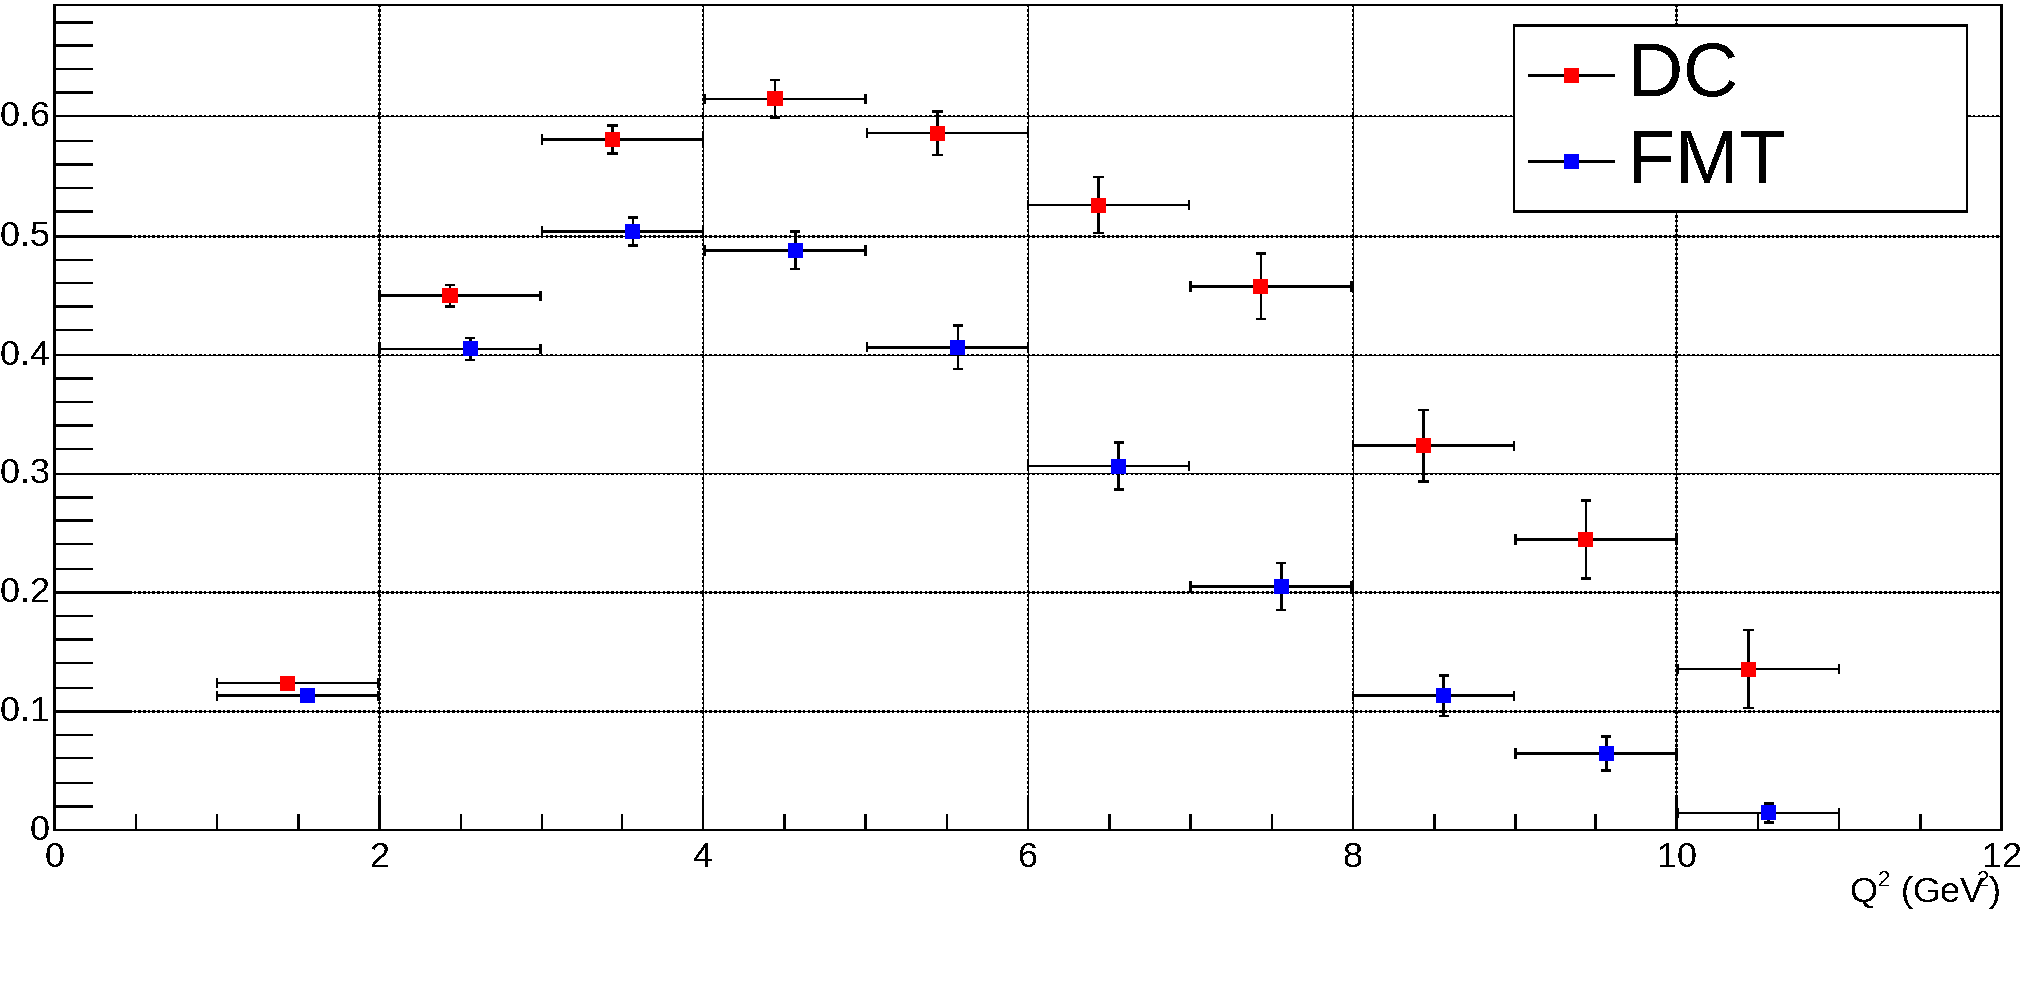
\includegraphics[width=\textwidth]{21q2_acc.pdf}
            \caption{$Q^2$ acceptance.}
            \label{fig::14.21::q2_acc}
        \end{subfigure}
        \hfill
        % nu.
        \begin{subfigure}[b]{\textwidth}
            \centering
            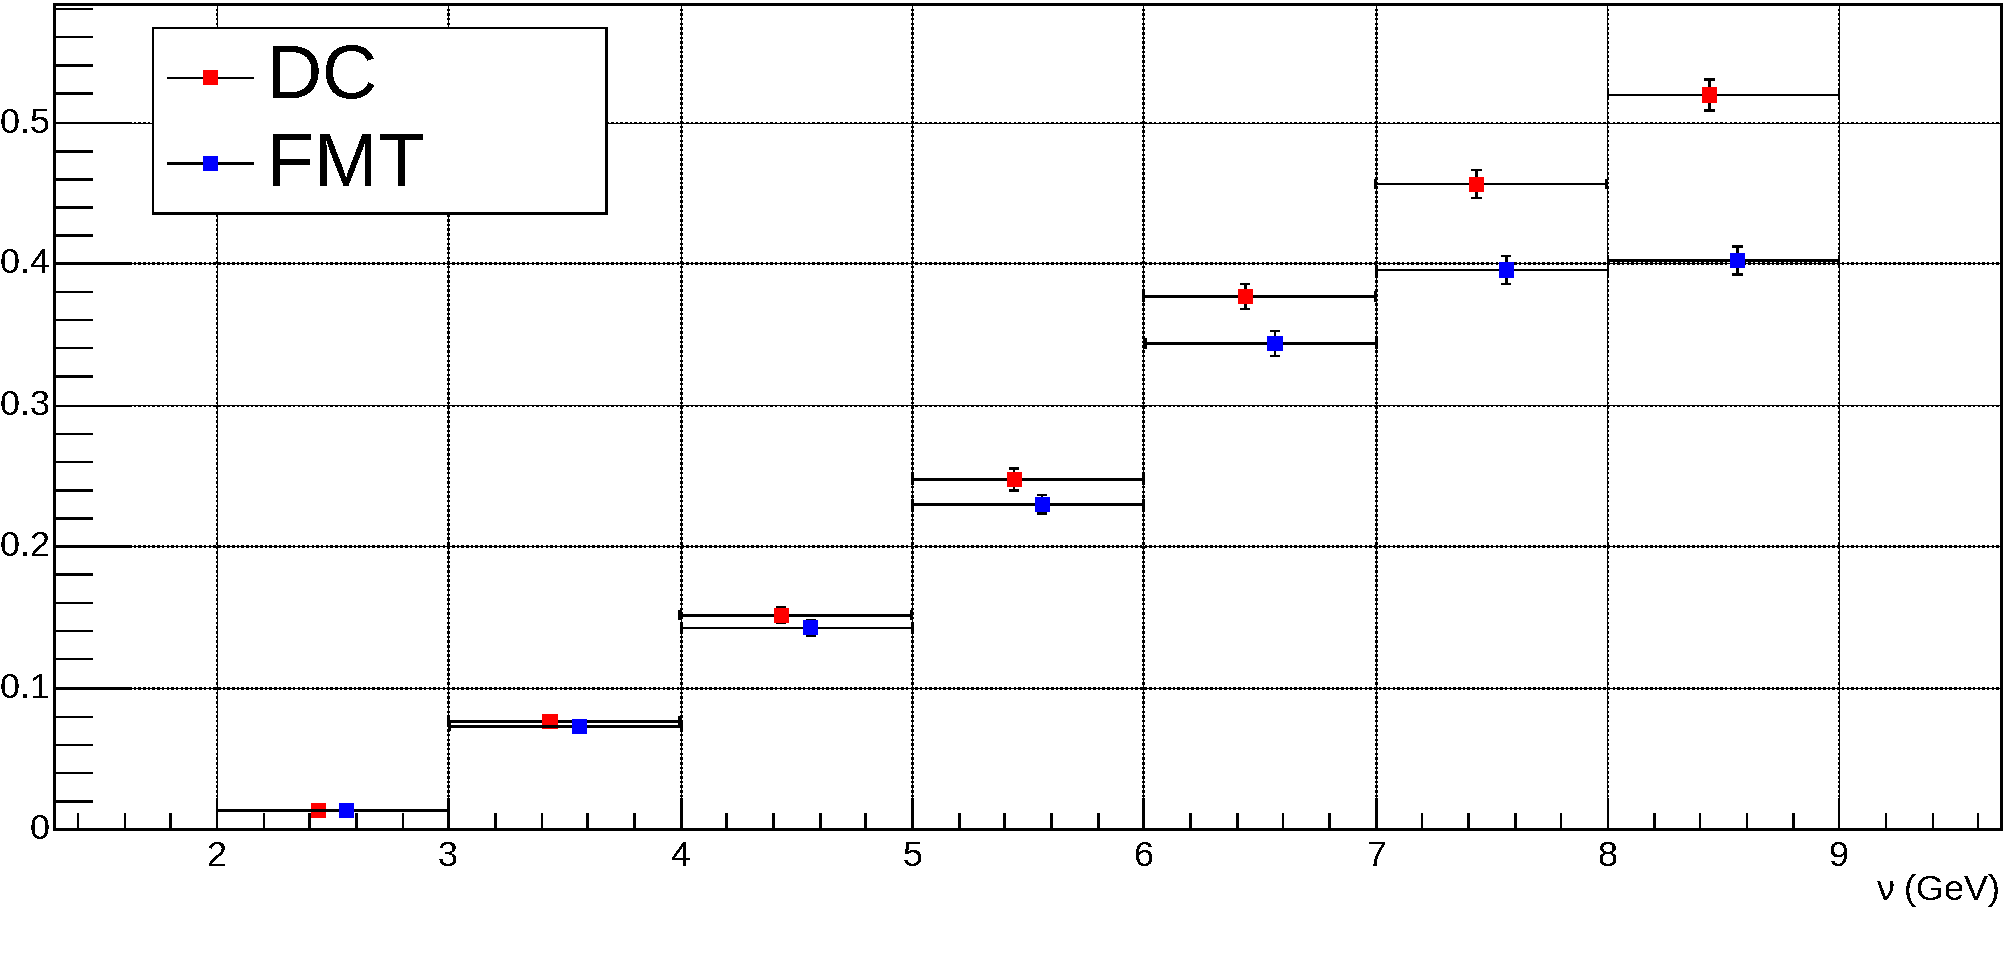
\includegraphics[width=\textwidth]{21nu_acc.pdf}
            \caption{$\nu$ acceptance.}
            \label{fig::14.21::nu_acc}
        \end{subfigure}
        \caption[$e^-$ variables acceptance]
        {$e^-$ variables acceptance.
        $\nu$ is integrated in \ref{fig::14.21::q2_acc}, and $Q^2$ is integrated in \ref{fig::14.21::nu_acc}.
        The bin markers are slightly shifted in $x$ to improve legibility.}
        \floatfoot{Source: Own elaboration, using the \href{https://github.com/bleaktwig/clas12-rge-analysis}{clas12-rge-analysis} software.}
        \label{fig::14.21::electron_acc}
    \end{figure}

    \begin{figure}
        \centering
        % phi vs. theta.
        \begin{subfigure}[b]{\textwidth}
            \centering
            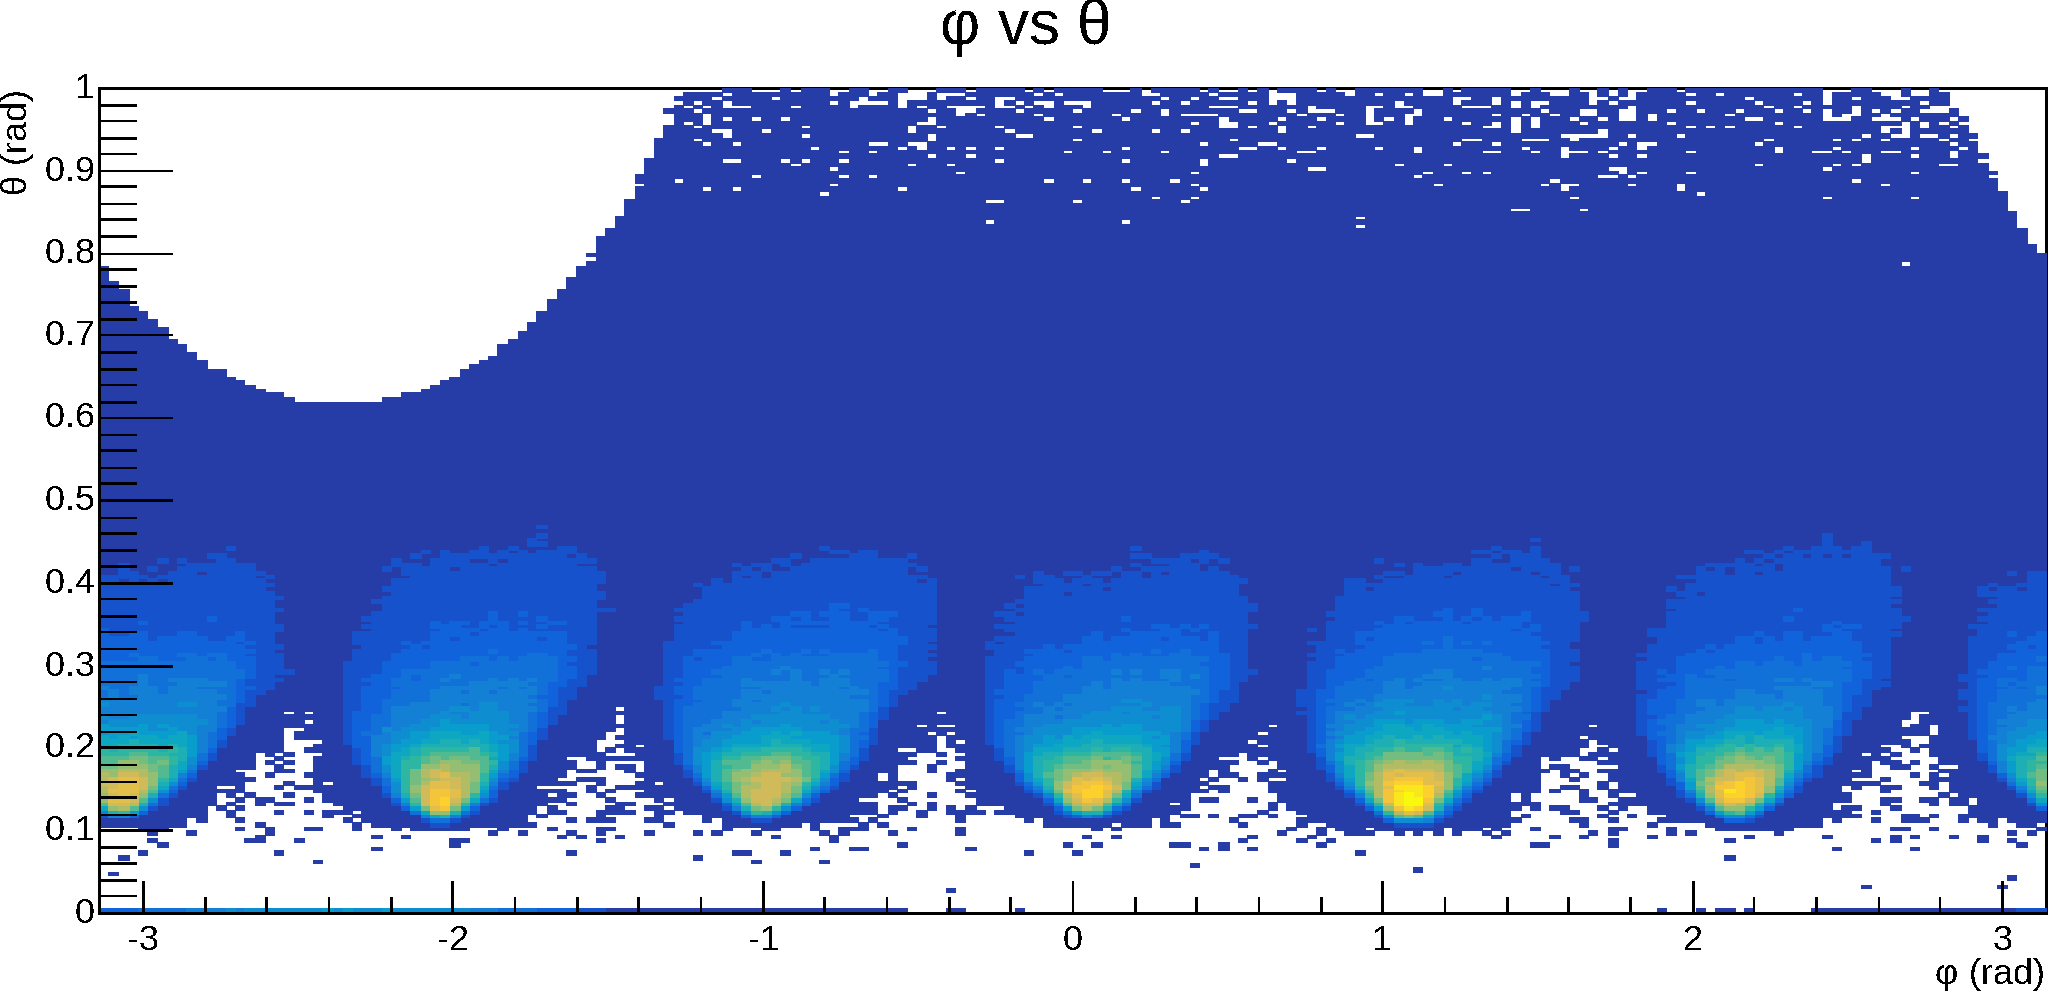
\includegraphics[width=\textwidth]{21phi_theta_neg.pdf}
            \caption[$\phi$ vs. $\theta$ for negative particles]
            {$\phi$ vs. $\theta$ for negative particles detected by DC.}
            \label{fig::14.21::phi_theta_neg}
        \end{subfigure}
        % theta.
        \begin{subfigure}[b]{\textwidth}
            \centering
            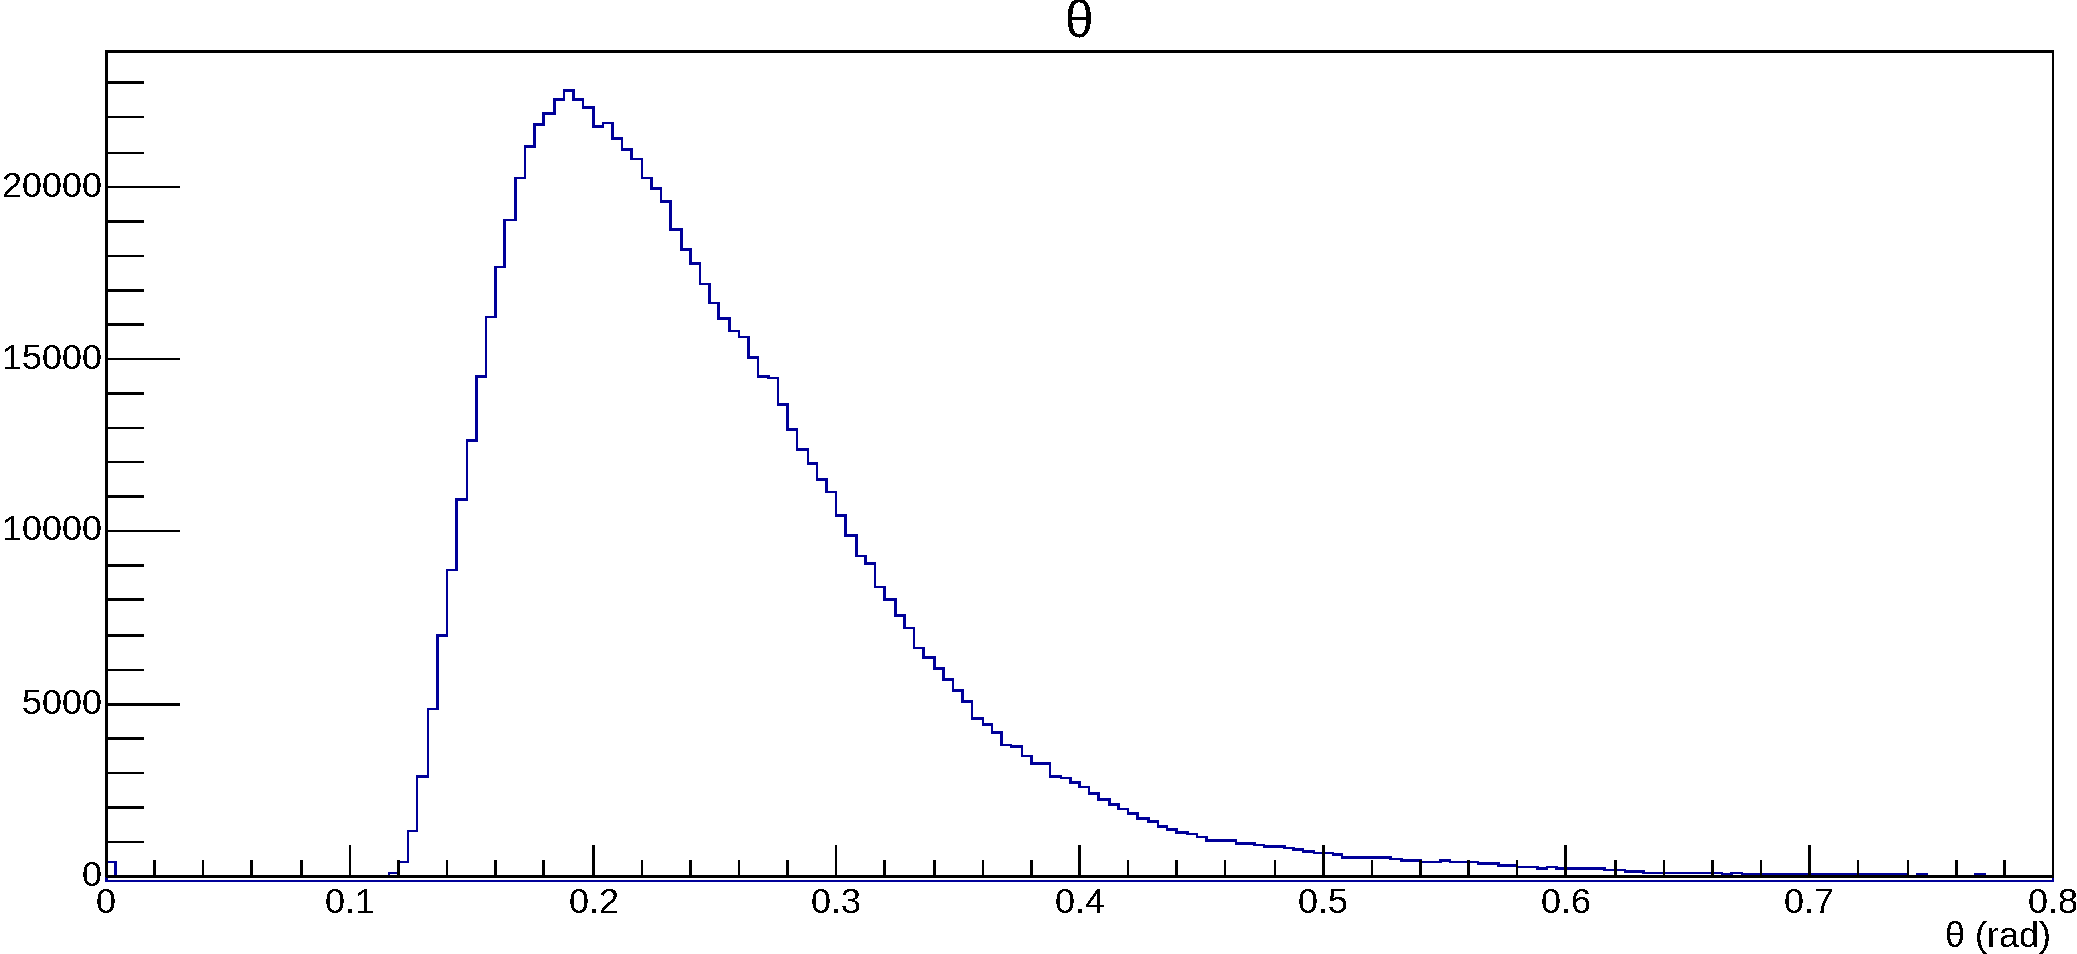
\includegraphics[width=\textwidth]{21theta_neg.pdf}
            \caption[$\theta$ for negative particles]
            {$\theta$ for negative particles detected by DC.}
            \label{fig::14.21::theta_neg}
        \end{subfigure}
        \caption[$\theta$ study for negative particles]
        {$\theta$ study for negative particles.
        Simulated RG-F target.}
        \floatfoot{Source: Own elaboration, using the \href{https://github.com/bleaktwig/clas12-rge-analysis}{clas12-rge-analysis} software.}
        \label{fig::14.21::theta_study_neg}
    \end{figure}

    % Q2.
    In Equation \eqref{eq::13.23::q2}, it can be observed that $Q^2$ has a quadratic dependence on the scattering angle $\theta_C$ of the scattered electrons.%, particularly for small angles.
    Hence, it is important to understand the $\theta$ acceptance of CLAS12 in order to distinguish the geometric effect related to $\theta$ from the inherent $Q^2$ acceptance of the FD.
    Figure \ref{fig::14.21::theta_study_neg} illustrates this dependence for negative particles.

    The triangular shape of each DC sector, combined with the inbending tracks resulting from the negative torus field, leads to a significantly low acceptance at low $\theta$ angles.
    When integrating across $\phi$, this results in a low $\theta$ efficiency for $\theta \lsim 0.15$ radians.
    Referring back to the $Q^2$ plot in Figure \ref{fig::14.21::q2_acc}, the decrease in $Q^2$ acceptance between 1 and 4 $GeV^2$ can be clearly attributed to this geometric effect, which is purely of a geometric nature.

    % nu
    On the other hand, since $\nu$ does not exhibit a direct correlation with $\theta_C$ (as indicated by Equation \eqref{eq::13.23::nu}), we can assume that the acceptance observed in Figure \ref{fig::14.21::nu_acc} is intrinsic to the detector.

    % !TEX root = ../main.tex
\subsubsection{Hadronic Variables}
\label{14.22::hadronic_variables}
    Next, we'll look at $z_h$, $p_T^2$, and $\phi_{PQ}$ acceptances for $e^-\pi^+$ and $e^-\pi^-$.
    It's worth noting that these acceptances are lower than those for electron variables.
    This is to be expected, since they require both the trigger electron and at least one hadron to be accepted by the detector, as is seen also on their efficiencies, as presented in Table \ref{tab::14.14::fmt_efficiency_study}

    \textbf{TODO. Say something?}

    We can see $z_h$ acceptance in Figure \textbf{TODO}, where... (TODO).

    Next, $p_T^2$ acceptance is presented in Figure \textbf{TODO}, where we see that... (TODO).

    Finally, $\phi_{PQ}$ acceptance is studied in Figure \textbf{TODO}.
    Here, we see... (TODO).

    % zh.
    \begin{figure}
        \centering
        % pi+.
        \begin{subfigure}[b]{0.49\textwidth}
            \centering
            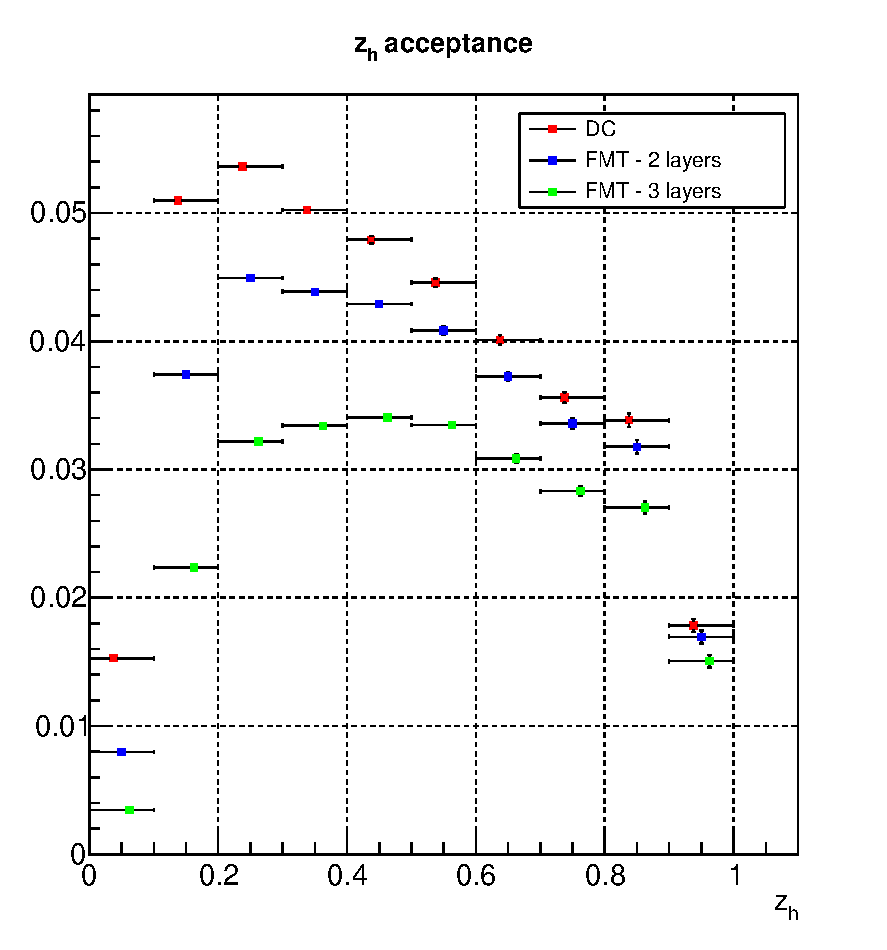
\includegraphics[width=\textwidth]{22zh_acc_211.pdf}
            \caption{$z_h$ acceptance for $e^-\pi^+$.}
            \label{fig::14.22::zh_acc_211}
        \end{subfigure}
        \hfill
        % pi-.
        \begin{subfigure}[b]{0.49\textwidth}
            \centering
            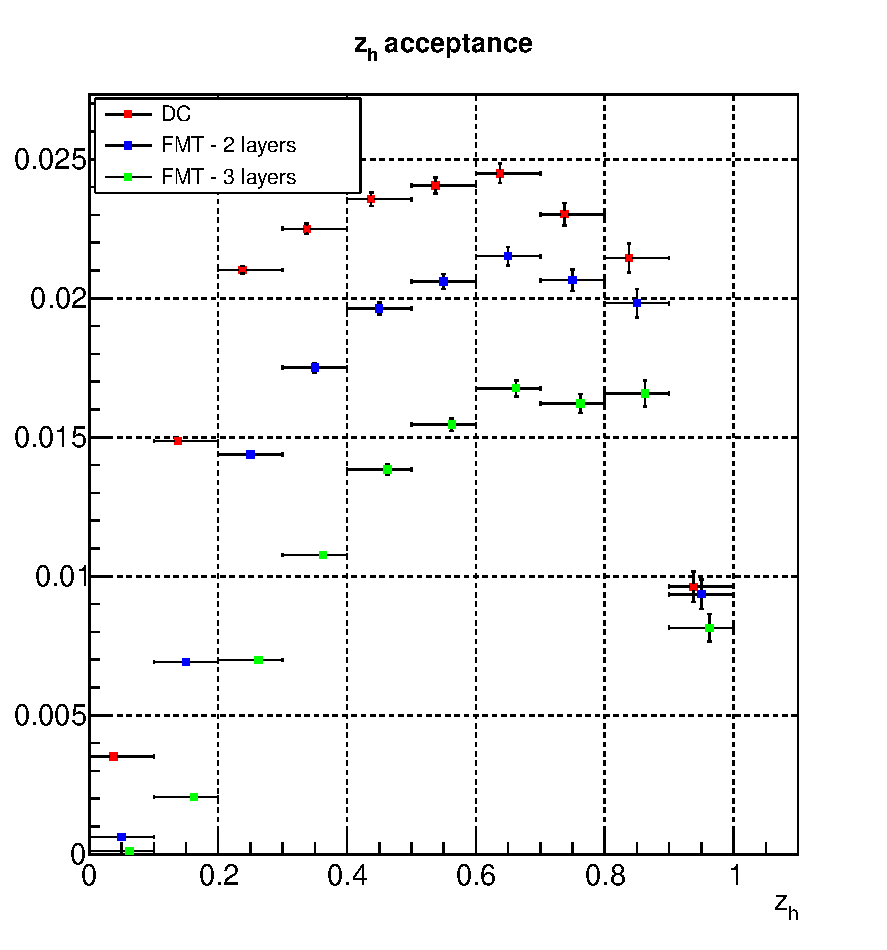
\includegraphics[width=\textwidth]{22zh_acc_-211.pdf}
            \caption{$z_h$ acceptance for $e^-\pi^-$.}
            \label{fig::14.22::zh_acc_-211}
        \end{subfigure}
        \caption[$z_h$ acceptance.]{$z_h$ acceptance for $e^-\pi^+$ and $e^-\pi^-$.
        All electron and other hadronic variables are integrated in both plots.
        The bin markers are slightly shifted in $x$ to improve legibility.
        Source: Own elaboration, using the \href{https://github.com/bleaktwig/clas12-rge-analysis}{clas12-rge-analysis} software.}
        \label{fig::14.22::zh_acc}
    \end{figure}

    % Pt2.
    \begin{figure}
        \centering
        % pi+.
        \begin{subfigure}[b]{0.49\textwidth}
            \centering
            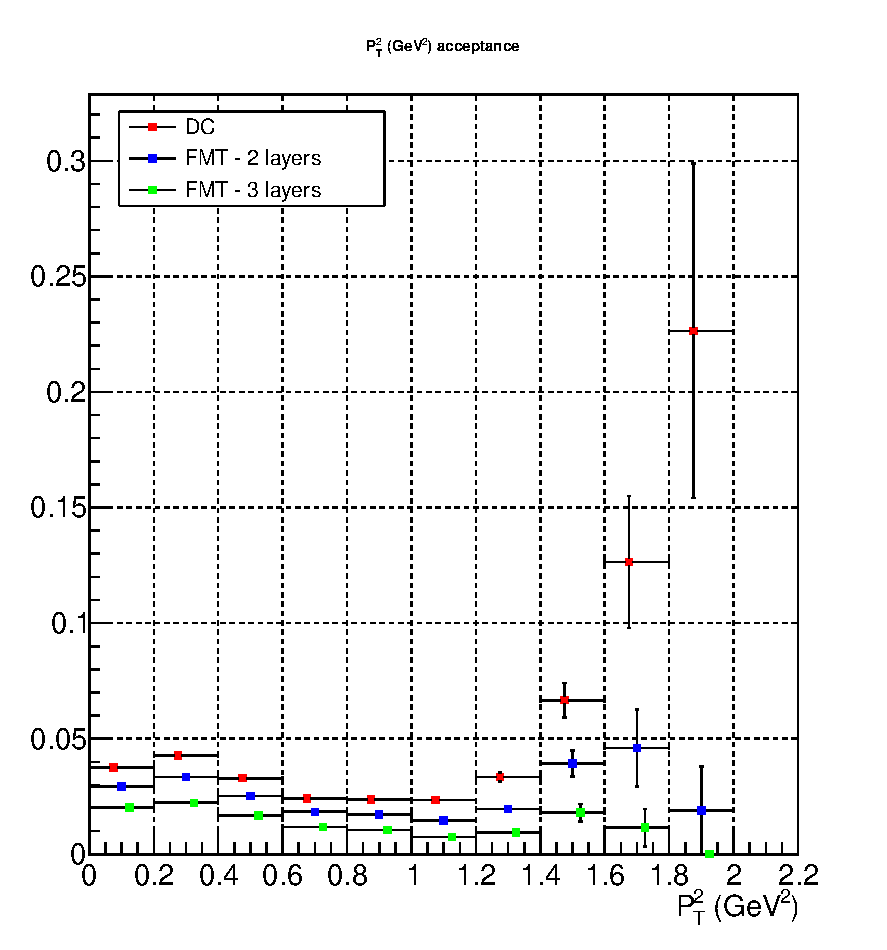
\includegraphics[width=\textwidth]{22pt2_acc_211.pdf}
            \caption{$p_T^2$ acceptance for $e^-\pi^+$.}
            \label{fig::14.22::pt2_acc_211}
        \end{subfigure}
        \hfill
        % pi-.
        \begin{subfigure}[b]{0.49\textwidth}
            \centering
            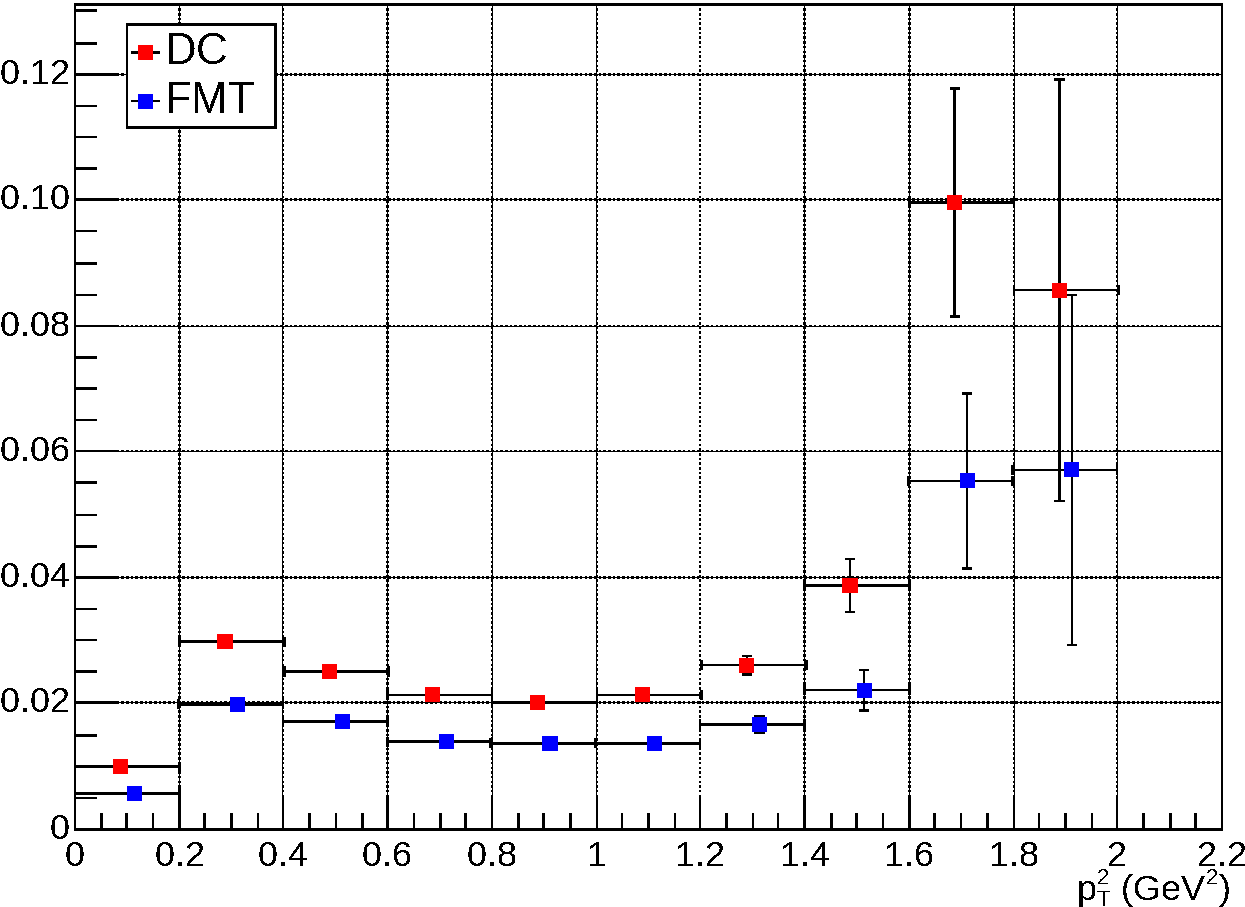
\includegraphics[width=\textwidth]{22pt2_acc_-211.pdf}
            \caption{$p_T^2$ acceptance for $e^-\pi^-$.}
            \label{fig::14.22::pt2_acc_-211}
        \end{subfigure}
        \caption[$p_T^2$ acceptance.]{$p_T^2$ acceptance for $e^-\pi^+$ and $e^-\pi^-$.
        All electron and other hadronic variables are integrated in both plots.
        The bin markers are slightly shifted in $x$ to improve legibility.
        Source: Own elaboration, using the \href{https://github.com/bleaktwig/clas12-rge-analysis}{clas12-rge-analysis} software.}
        \label{fig::14.22::pt2_acc}
    \end{figure}

    % phipq.
    \begin{figure}
        \centering
        % pi+.
        \begin{subfigure}[b]{0.49\textwidth}
            \centering
            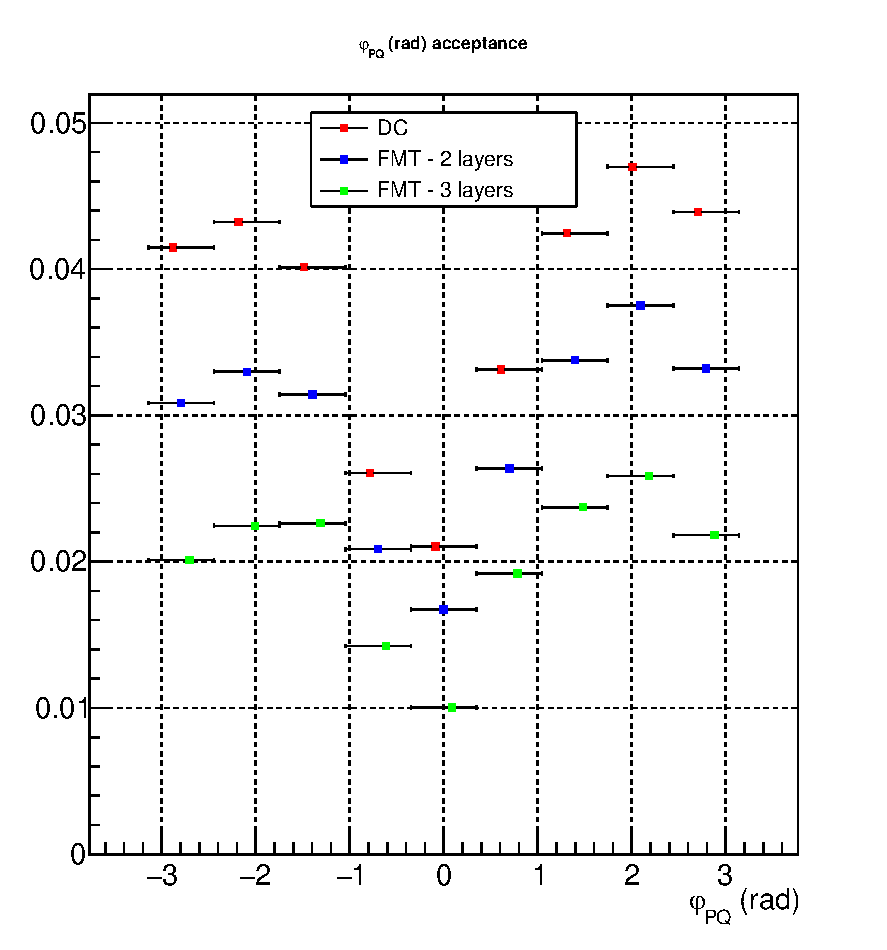
\includegraphics[width=\textwidth]{22phipq_acc_211.pdf}
            \caption{$\phi_{PQ}$ acceptance for $e^-\pi^+$.}
            \label{fig::14.22::phipq_acc_211}
        \end{subfigure}
        \hfill
        % pi-.
        \begin{subfigure}[b]{0.49\textwidth}
            \centering
            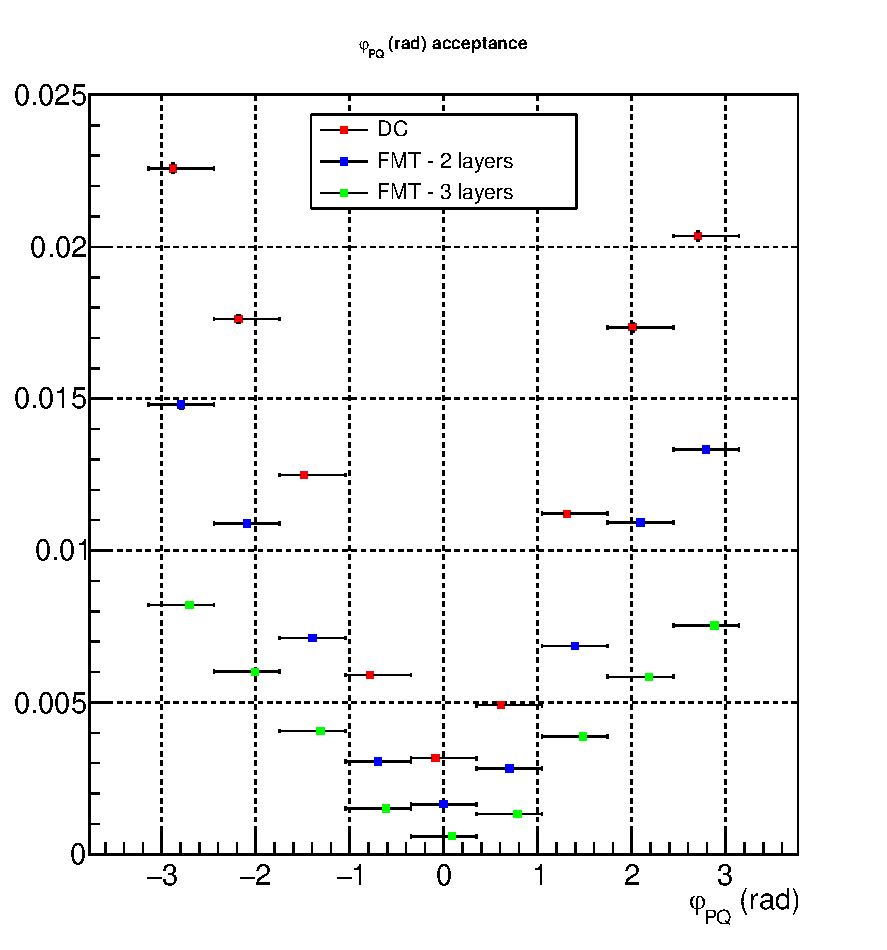
\includegraphics[width=\textwidth]{22phipq_acc_-211.pdf}
            \caption{$\phi_{PQ}$ acceptance for $e^-\pi^-$.}
            \label{fig::14.22::phipq_acc_-211}
        \end{subfigure}
        \caption[$\phi_{PQ}$ acceptance.]{$\phi_{PQ}$ acceptance for $e^-\pi^+$ and $e^-\pi^-$.
        All electron and other hadronic variables are integrated in both plots.
        The bin markers are slightly shifted in $x$ to improve legibility.
        Source: Own elaboration, using the \href{https://github.com/bleaktwig/clas12-rge-analysis}{clas12-rge-analysis} software.}
        \label{fig::14.22::phipq_acc}
    \end{figure}

